\documentclass{article}[18pt]
\usepackage{../../../../format}
\lhead{Software Engineering - HCI}


\begin{document}
\begin{center}
\underline{\huge HCI 1}
\end{center}
\begin{defin}[HCI]
This discipline concerned with the design, evaluation and implementation of interactive computer systems for human use and with the study of major phenomena surrounding them
\end{defin}
Objectives of HCI are
\begin{itemize}
	\item To provide an understanding of both the human user and the computer system, in an effort to make interactions between the two easier and more satisfying
	\item However the emphasis should always be on the user
\end{itemize}
\textbf{User}
\begin{itemize}
	\item An individual user, a group of users working together or a sequence of users in an organisation dealing with some part of a process or task
\end{itemize}
\textbf{Computer}
\begin{itemize}
	\item Technology ranging from desktop to large scale systems, or control/embedded systems
\end{itemize}
\textbf{Interaction}
\begin{itemize}
	\item Communication between the user and computer in a direct or indirect manner
\end{itemize}
\section{What is involved}
\begin{itemize}
	\item Study of humans using interfaces
	\item Development of new applications/systems to support user's activities
	\item Development of new devices and tools for users
	\item Develop usable products
	\begin{itemize}
		\item Easy to learn
		\item Effective to use
		\item Provide an enjoyable/satisfying experience
	\end{itemize}
\end{itemize}
\section{Why should you be concerned with HCI}
Increasingly becomes a matter of law\\
\\
National health ans safety standards constrain employers to provide their workforce with usable computer systems\\
\\
EC directive 90/270/EEC - when designing, selecting, commissioning or modifying software
\begin{itemize}
	\item Is suitable to task
	\item Is easy to use and adaptable to the user's knowledge and experience
	\item It provides feedback on performance
	\item It displays information in a format and at a pace that is adapted to the user
	\item It conforms to the "principle of software ergonomics"
\end{itemize}
Designers and employers cannot afford to ignore the user
\section{Principles for supporting HCI}
\begin{itemize}
	\item Listening to what people want and getting them involved in design
	\item Using tried and tested user-based techniques during the design process
	\item Thinking through what might provide quality user experiences
	\item Considering what might help people with the way they currently do things
	\item Taking into account what people are good and bad at
\end{itemize}
\section{Avoiding problematic design}
Take into account
\begin{itemize}
	\item Who the users are
	\item What activities are being carried out
	\item Where the interaction is taking place
\end{itemize}
\section{Memory and mental models}
\subsection{Multi-store memory}
Sensory memory
\begin{itemize}
	\item Iconic, Echoic, Haptic
	\item Hold info for a few tenths
	\item Attention passes info to short term memory
\end{itemize}
Short term memory store
\begin{itemize}
	\item Scratch pad for temporary recall of info
	\item Holds info for a few seconds (then decays)
	\item Has limited capacity 7+-2 digits for information
	\item Passed to long term memory via rehearsal 
\end{itemize}
Permanent long-term memory store
\begin{itemize}
	\item Everything we "know"
	\item Factual knowledge
	\item Experimental knowledge
	\item Procedural rules of behaviour etc.
	\item Hold information "indefinitely"
	\item Episodic - memory of events and experience in serial form
	\item Semantic - uses structure to store information derived from episodic memory list
\end{itemize}
\subsection{Mental models}
An explanation in what someone's though process for how something works in the real world\\
\\
A mental model is what the user believes about the system at hand\\
\\
Knowledge is sometimes described as a mental model
\begin{itemize}
	\item How to use the system (what to do next)
	\item What to do with unfamiliar systems or unexpected situations (how the system works)
\end{itemize}
People make inferences using mental models of how to carry out tasks
\begin{center}
	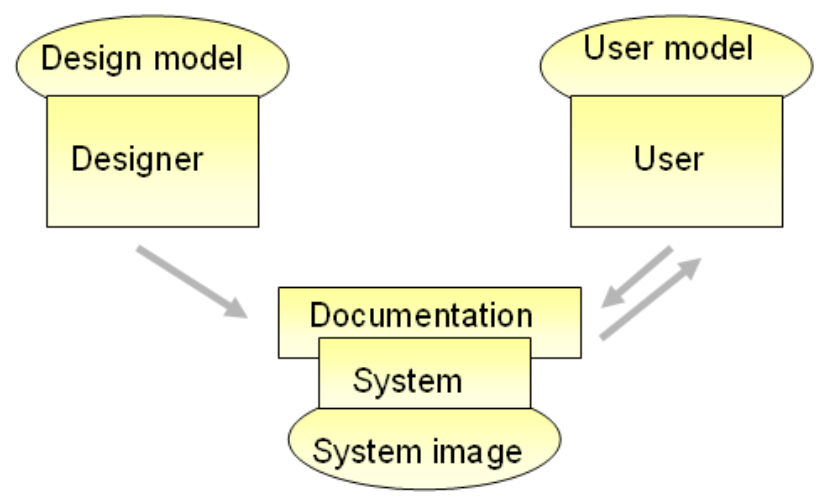
\includegraphics[scale=0.7]{Conceptual}
\end{center}
\subsection{What to do in HCI design}
Educate the user to build correct mental models\\
\\
Transparency:
\begin{itemize}
	\item Useful feedback in response to user input
	\item Easy to understand and intuitive ways of interacting with the system
	\item Provide the right kind and level of info in the form of:
	\begin{itemize}
		\item Clear and easy to follow instructions
		\item Appropriate online help and tutorials
		\item Context sensitive guidance for users, set at their level of experience 
	\end{itemize}
\end{itemize}
\section{HCI, science or craft?}
Both - artistically pleasing and capable of fulfilling the tasks required
\end{document}